%\begin{frame}{Test Results}{Linear model}
%	\begin{itemize}
%		\item A text
%	\end{itemize}
%\end{frame}

%%%%%%%%%%%%%%%%

\begin{frame}{Test Results}{VTS: 16 m/s - LQI vs. FLC vs. detuned FLC}
	\begin{columns}
		\begin{column}{.25\linewidth}
			\small{
				\setbeamercolor{normal text}{fg=blue}\usebeamercolor*{normal text}
			BLUE
				\setbeamercolor{normal text}{fg=black}\usebeamercolor*{normal text}
				: LQI controller
			
			\smallskip
			\setbeamercolor{normal text}{fg=red}\usebeamercolor*{normal text}
			RED
			\setbeamercolor{normal text}{fg=black}\usebeamercolor*{normal text}
			: Detuned FLC PI controller
			
			\smallskip
			\setbeamercolor{normal text}{fg=yellow}\usebeamercolor*{normal text}
			YELLOW
			\setbeamercolor{normal text}{fg=black}\usebeamercolor*{normal text}
			: FLC
			}
			
			\begin{table}[t]
				\centering
				\label{tab:del}
				\resizebox{1.1\textwidth}{!}{ %
					\begin{tabular}{@{}|lll|@{}}
						\toprule
						\multicolumn{3}{|c|}{1 Hz damage equivalent loads}                                                                     \\ \midrule
						\multicolumn{1}{|l|}{LQI}                           & \multicolumn{1}{l|}{FLC detuned} & FLC                           \\ \midrule
						\multicolumn{1}{|l|}{\cellcolor[HTML]{9AFF99}21760} & \multicolumn{1}{l|}{25099}       & \cellcolor[HTML]{FFCCC9}81343 \\ \bottomrule
					\end{tabular}
				} %
			\end{table}
			\begin{table}[t]
				\centering
				\label{tab:pitch_sum}
				\resizebox{1.2\textwidth}{!}{ %
					\begin{tabular}{@{}|llll|@{}}
						\toprule
						\multicolumn{4}{|c|}{Blade pitch actuation sums}                                                                                                   \\ \midrule
						\multicolumn{1}{|l|}{}           & \multicolumn{1}{l|}{LQI}   & \multicolumn{1}{l|}{FLC detuned}                   & FLC                           \\ \midrule
						\multicolumn{1}{|l|}{Unfiltered} & \multicolumn{1}{l|}{169.9} & \multicolumn{1}{l|}{\cellcolor[HTML]{9AFF99}103.3} & \cellcolor[HTML]{FFCCC9}716.5 \\ \midrule
						\multicolumn{1}{|l|}{Filtered}   & \multicolumn{1}{l|}{67.6}  & \multicolumn{1}{l|}{\cellcolor[HTML]{9AFF99}63.7}  & \cellcolor[HTML]{FFCCC9}557.7 \\ \bottomrule
					\end{tabular}
				} %
			\end{table}
		\end{column}
		\begin{column}{.75\linewidth}
			\begin{figure}[h]
				\centering
				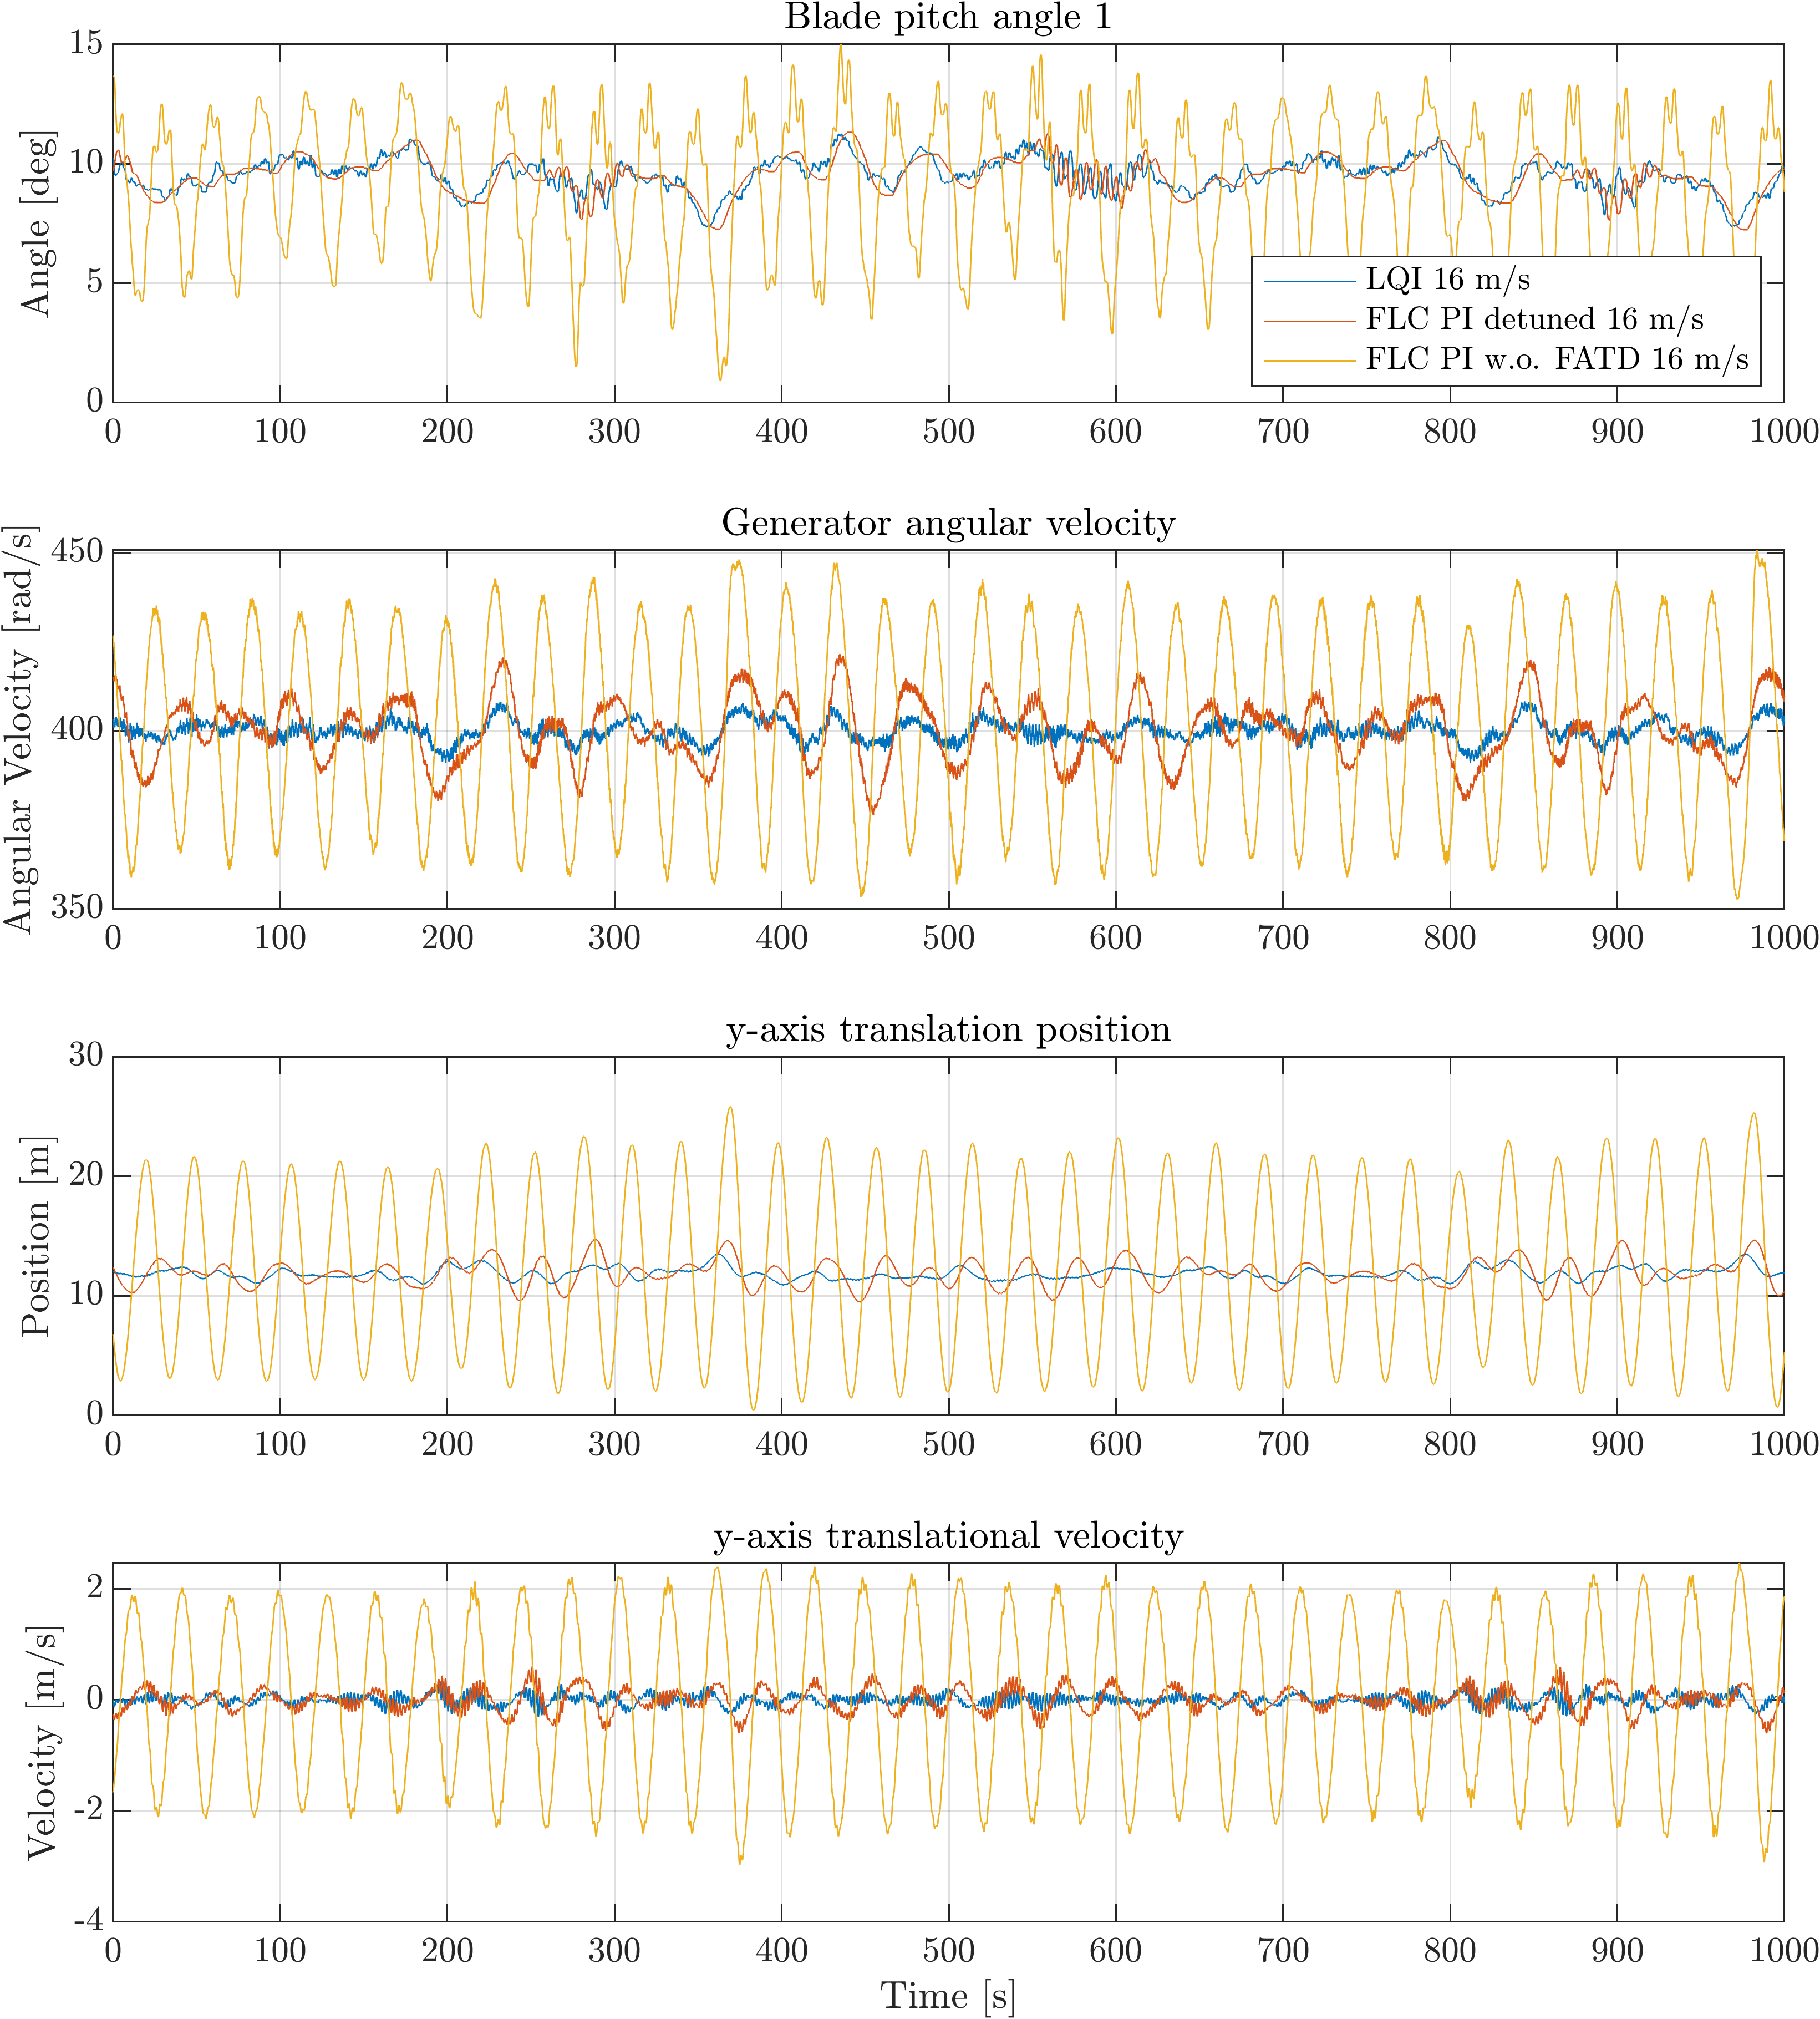
\includegraphics[width=0.9\linewidth]{../Graphics/TestResults/VTSplotting/3_th_w_py_vy.png}
				\label{fig:vts_3_th_w_py_vy}
			\end{figure}
		\end{column}
	\end{columns}
\end{frame}


%%%%%%%%%%%%%%%%

\begin{frame}{Test Results}{VTS: 16 m/s - LQI vs. detuned FLC}
	\begin{columns}
		\begin{column}{.25\linewidth}

			\begin{align*}
				|e_\omega| & < 10 \text{\small{ rpm}} \\
				|\hat p_y| & < 1 \text{\small{ m}}
			\end{align*}

			\begin{table}[t]
				\centering
				\label{tab:del2}
				\resizebox{1.1\textwidth}{!}{ %
				\begin{tabular}{@{}|lll|@{}}
					\toprule
					\multicolumn{3}{|c|}{1 Hz damage equivalent loads}                                                                     \\ \midrule
					\multicolumn{1}{|l|}{LQI}                           & \multicolumn{1}{l|}{FLC detuned} & FLC                           \\ \midrule
					\multicolumn{1}{|l|}{\cellcolor[HTML]{9AFF99}21760} & \multicolumn{1}{l|}{25099}       & \cellcolor[HTML]{FFCCC9}81343 \\ \bottomrule
				\end{tabular}
				} %
			\end{table}
			\begin{table}[t]
				\centering
				\label{tab:pitch_sum2}
				\resizebox{1.2\textwidth}{!}{ %
					\begin{tabular}{@{}|llll|@{}}
						\toprule
						\multicolumn{4}{|c|}{Blade pitch actuation sums}                                                                                                   \\ \midrule
						\multicolumn{1}{|l|}{}           & \multicolumn{1}{l|}{LQI}   & \multicolumn{1}{l|}{FLC detuned}                   & FLC                           \\ \midrule
						\multicolumn{1}{|l|}{Unfiltered} & \multicolumn{1}{l|}{169.9} & \multicolumn{1}{l|}{\cellcolor[HTML]{9AFF99}103.3} & \cellcolor[HTML]{FFCCC9}716.5 \\ \midrule
						\multicolumn{1}{|l|}{Filtered}   & \multicolumn{1}{l|}{67.6}  & \multicolumn{1}{l|}{\cellcolor[HTML]{9AFF99}63.7}  & \cellcolor[HTML]{FFCCC9}557.7 \\ \bottomrule
					\end{tabular}
				} %
			\end{table}
		\end{column}
	
		\begin{column}{.75\linewidth}
			\begin{figure}[h]
				\centering
				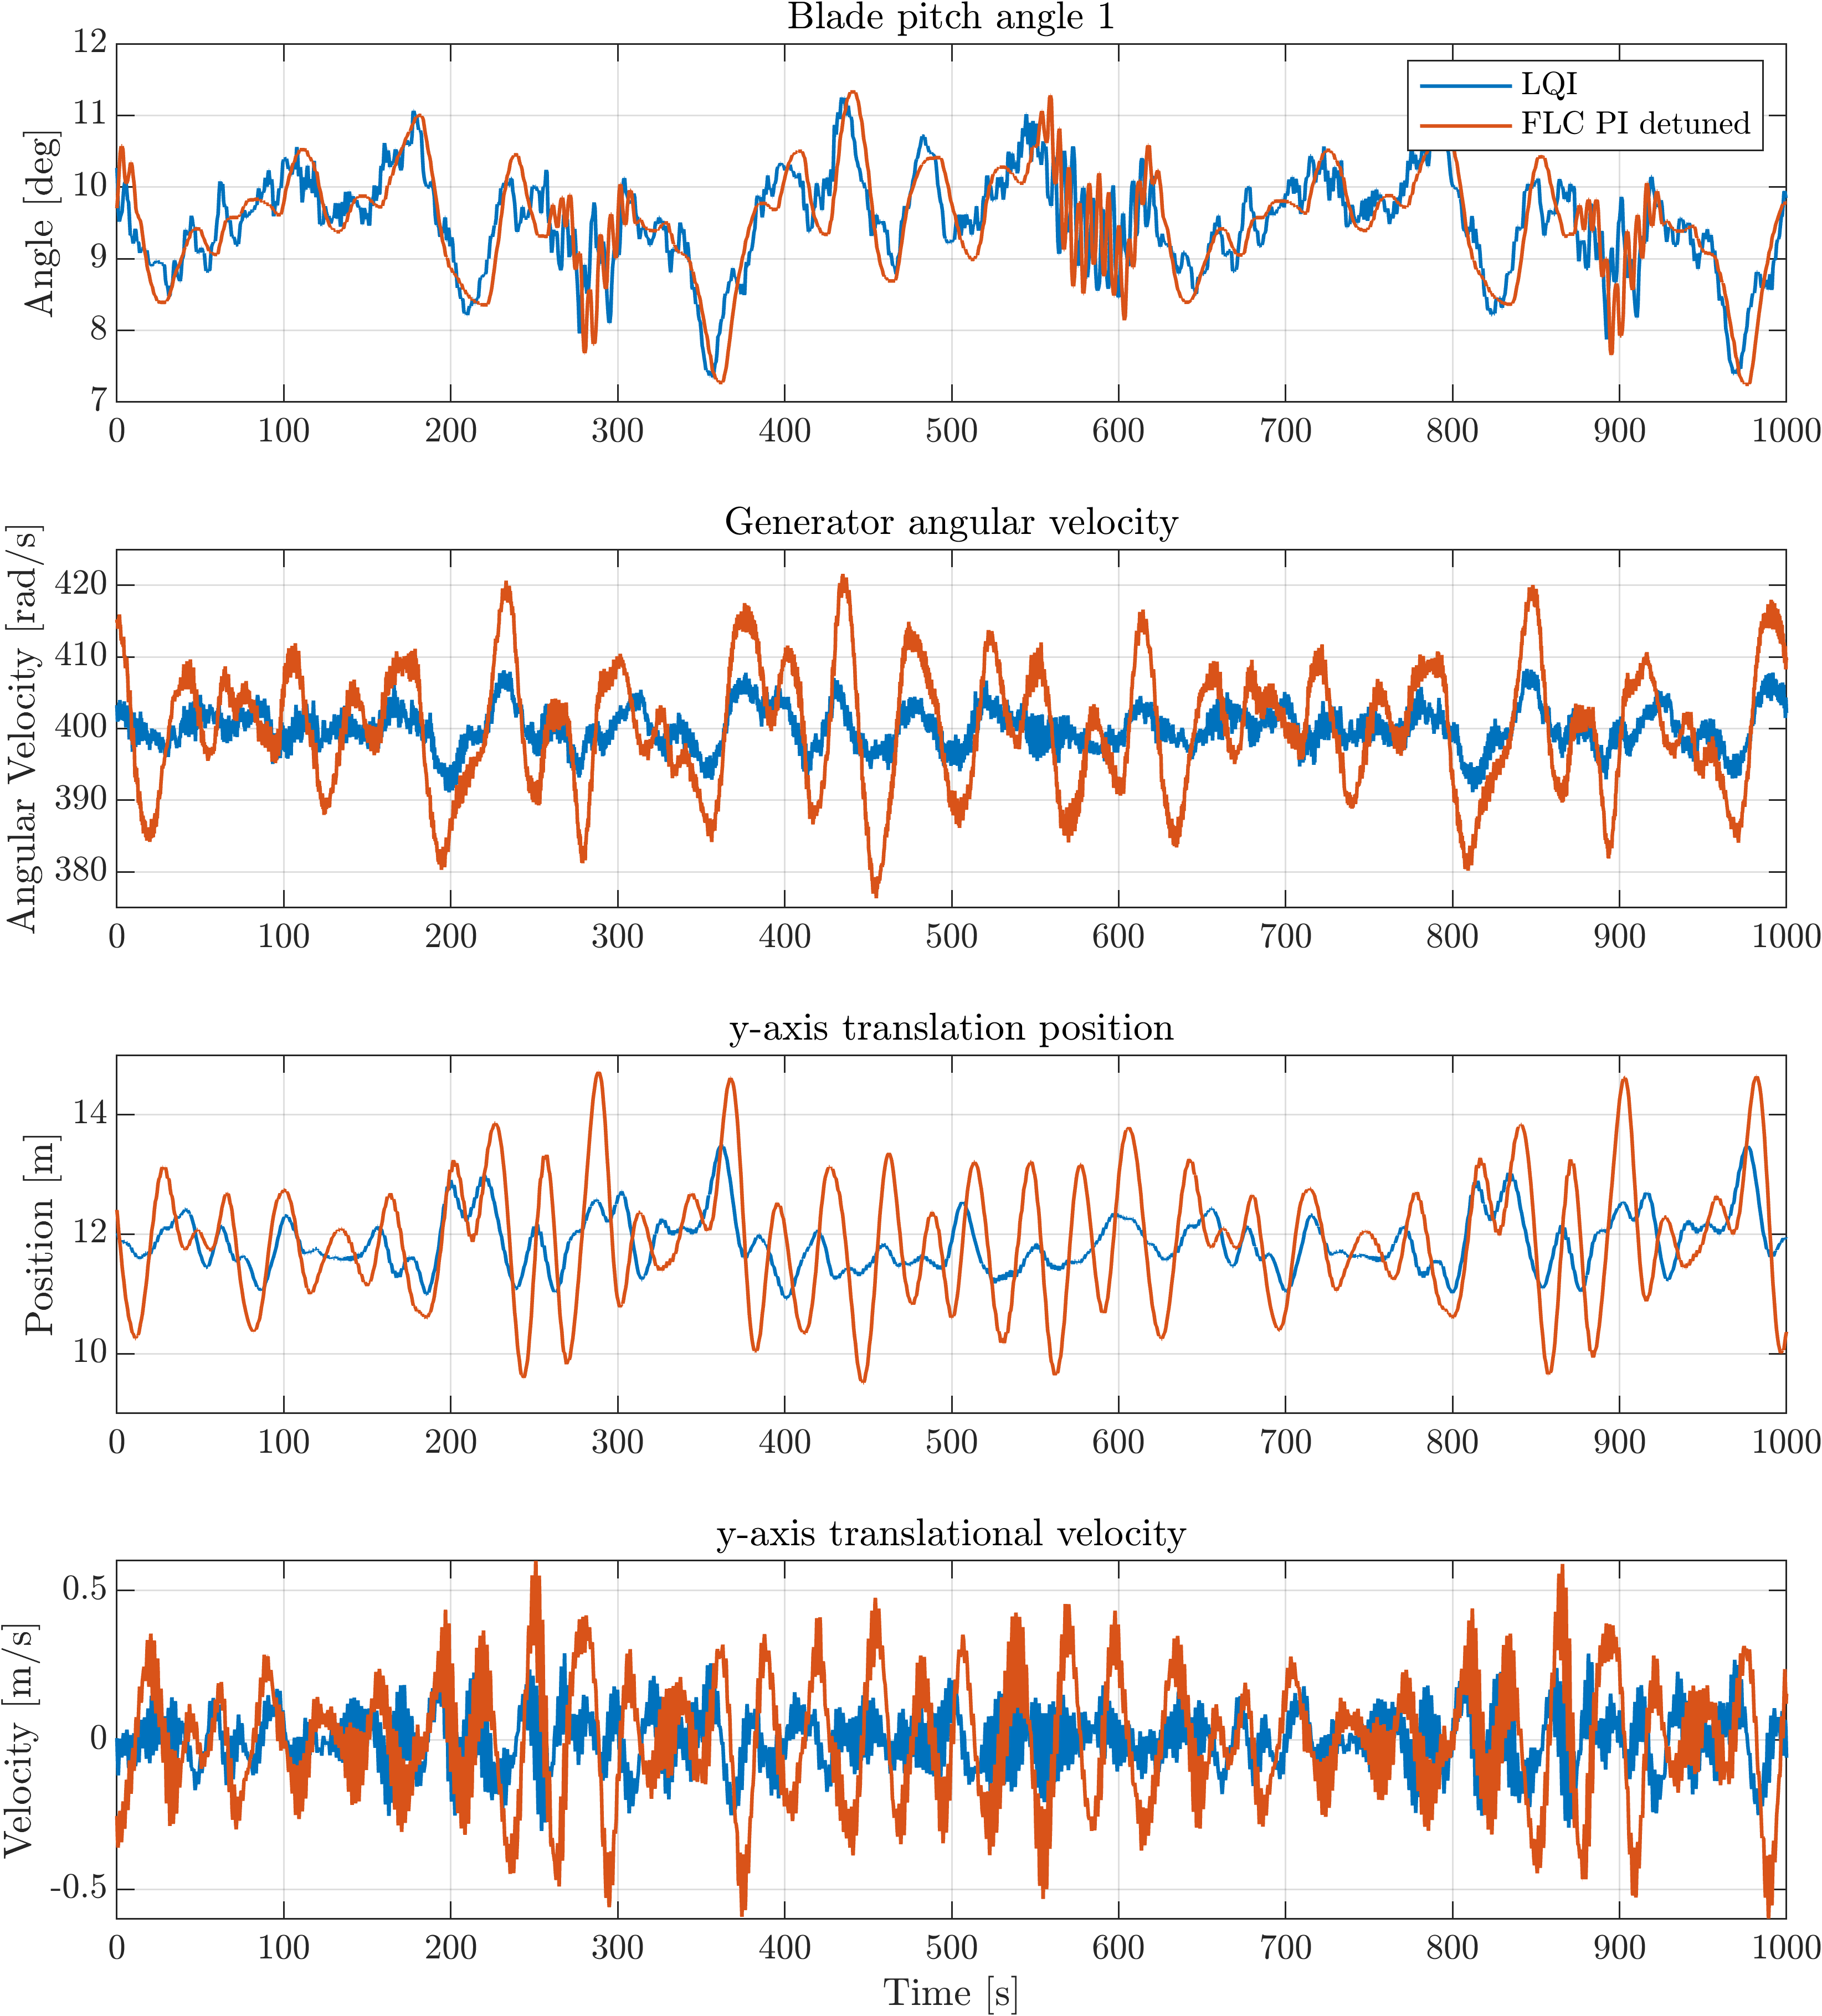
\includegraphics[width=0.9\linewidth]{../Graphics/TestResults/VTSplotting/10_th_w_py_vy.png}
				\label{fig:vts_10_th_w_py_vy}
			\end{figure}
		\end{column}
	\end{columns}	
	
	
\end{frame}

%%%%%%%%%%%%%%%%
%
%\begin{frame}{Test Results}{VTS: 12, 16 and 26 m/s - DELs}
%	
%	\begin{table}[ht]
%		\centering
%		\caption{1 Hz damage equivalent loads of LQI controllers}
%		\label{tab:del_lqi}
%		\begin{tabular}{@{}|llll|@{}}
%			\toprule
%			\multicolumn{4}{|c|}{1 Hz damage equivalent loads of LQI controllers}                                                                                                                                \\ \midrule
%			\multicolumn{1}{|l|}{}              & \multicolumn{1}{l|}{LQI OP 12}                                            & \multicolumn{1}{l|}{LQI OP 16}                     & LQI OP 26                     \\ \midrule
%			\multicolumn{1}{|l|}{Wind speed 12} & \multicolumn{1}{l|}{\cellcolor[HTML]{FFCCC9}{\color[HTML]{333333} 24132}} & \multicolumn{1}{l|}{\cellcolor[HTML]{9AFF99}23127} & 23749                         \\ \midrule
%			\multicolumn{1}{|l|}{Wind speed 16} & \multicolumn{1}{l|}{\cellcolor[HTML]{FFCCC9}185830}                       & \multicolumn{1}{l|}{21760}                         & \cellcolor[HTML]{9AFF99}21525 \\ \midrule
%			\multicolumn{1}{|l|}{Wind speed 26} & \multicolumn{1}{l|}{\cellcolor[HTML]{FFCCC9}115800}                       & \multicolumn{1}{l|}{36366}                         & \cellcolor[HTML]{9AFF99}23515 \\ \bottomrule
%		\end{tabular}
%	\end{table}
%	
%\end{frame}
%
%%%%%%%%%%%%%%%%%
%
%\begin{frame}{Test Results}{VTS: 12, 16 and 26 m/s - Blade actuation sums}
%		
%	\begin{table}[ht]
%		\centering
%		\caption{Blade pitch actuation sums of LQI controllers}
%		\label{tab:pitch_sum_lqi}
%		\resizebox{0.75\textwidth}{!}{ %
%		\begin{tabular}{@{}|llll|@{}}
%			\toprule
%			\multicolumn{4}{|c|}{Blade pitch actuation sums of LQI controllers}                                                                                                           \\ \midrule
%			\multicolumn{1}{|l|}{}              & \multicolumn{1}{l|}{LQI OP 12}                     & \multicolumn{1}{l|}{LQI OP 16}                     & LQI OP 26                     \\ \midrule
%			\multicolumn{1}{|l|}{Wind Speed 12} & \multicolumn{1}{l|}{\cellcolor[HTML]{FFCCC9}186.4} & \multicolumn{1}{l|}{\cellcolor[HTML]{9AFF99}113.3} & 139.3                         \\ \midrule
%			\multicolumn{1}{|l|}{Wind Speed 16} & \multicolumn{1}{l|}{\cellcolor[HTML]{FFCCC9}8432}  & \multicolumn{1}{l|}{169.9}                         & \cellcolor[HTML]{9AFF99}132.8 \\ \midrule
%			\multicolumn{1}{|l|}{Wind Speed 26} & \multicolumn{1}{l|}{\cellcolor[HTML]{FFCCC9}12261} & \multicolumn{1}{l|}{1033.6}                        & \cellcolor[HTML]{9AFF99}795.6 \\ \bottomrule
%		\end{tabular}
%		} %
%	\end{table}
%	
%	\begin{table}[ht]
%		\centering
%		\caption{Filtered blade pitch actuation sums of LQI controllers}
%		\label{tab:filt_pitch_sum_lqi}
%		\resizebox{0.75\textwidth}{!}{ %
%		\begin{tabular}{@{}|llll|@{}}
%			\toprule
%			\multicolumn{4}{|c|}{Filtered blade pitch actuation sums}                                                                                                                        \\ \midrule
%			\multicolumn{1}{|l|}{}              & \multicolumn{1}{l|}{LQI OP 12}                     & \multicolumn{1}{l|}{LQI OP 16} & LQI OP 26                                            \\ \midrule
%			\multicolumn{1}{|l|}{Wind Speed 12} & \multicolumn{1}{l|}{\cellcolor[HTML]{9AFF99}115.6} & \multicolumn{1}{l|}{116.3}     & \cellcolor[HTML]{FFCCC9}{\color[HTML]{333333} 128.9} \\ \midrule
%			\multicolumn{1}{|l|}{Wind Speed 16} & \multicolumn{1}{l|}{\cellcolor[HTML]{9AFF99}63.1}  & \multicolumn{1}{l|}{67.6}      & \cellcolor[HTML]{FFCCC9}77.6                         \\ \midrule
%			\multicolumn{1}{|l|}{Wind Speed 26} & \multicolumn{1}{l|}{\cellcolor[HTML]{FFCCC9}205.2} & \multicolumn{1}{l|}{65.2}      & \cellcolor[HTML]{9AFF99}64.4                         \\ \bottomrule
%		\end{tabular}
%		} %
%	\end{table}
%	
%\end{frame}